\documentclass[conference]{IEEEtran}
\IEEEoverridecommandlockouts
% The preceding line is only needed to identify funding in the first footnote. If that is unneeded, please comment it out.
\usepackage{cite}
\usepackage{amsmath,amssymb,amsfonts}
\usepackage{algorithmic}
\usepackage{graphicx}
\usepackage{textcomp}
\usepackage{xcolor}
\usepackage{tikz}
\usetikzlibrary{arrows, positioning, shadows, shapes.geometric}

\def\BibTeX{{\rm B\kern-.05em{\sc i\kern-.025em b}\kern-.08em
    T\kern-.1667em\lower.7ex\hbox{E}\kern-.125emX}}
\begin{document}

\title{A Study on the Integration of Artificial Intelligence in Blockchain-Based Voting Systems\\}

\author{
    \IEEEauthorblockN{1\textsuperscript{st} Dr. Rajesh Kumar}
    \IEEEauthorblockA{\textit{Associate Professor} \\
        \textit{Vellore Institute of Technology}\\
        Chennai, India \\
        rajesh.kumar@vit.ac.in}
    \and
    \IEEEauthorblockN{2\textsuperscript{nd} Kakakarala Sreevallabh}
    \IEEEauthorblockA{\textit{Integrated M.Tech Software Engineering} \\
        \textit{Vellore Institute of Technology}\\
        Chennai, India \\
        sreevallabh.2022@vitstudent.ac.in}
    \and
    \IEEEauthorblockN{3\textsuperscript{rd} Aman Pandey}
    \IEEEauthorblockA{\textit{Integrated M.Tech Software Engineering} \\
        \textit{Vellore Institute of Technology}\\
        Chennai, India \\
        aman.pandey2022@vitstudent.ac.in}
}



\maketitle

\begin{abstract}
This paper presents a comprehensive study on the integration of artificial intelligence (AI) with blockchain technology to enhance electronic voting systems. Traditional voting methods face numerous challenges related to security, transparency, and efficiency that modern technology could potentially address. We examine the current state of both blockchain-based voting systems and AI applications in electoral contexts, identifying gaps and opportunities at their intersection. Through an extensive literature review, we analyze how AI can complement blockchain in areas such as voter authentication, fraud detection, and system optimization. We propose a conceptual framework illustrating potential integration points between these technologies and discuss possible applications including intelligent authentication, anomaly detection, decision support, and privacy-preserving analytics. The study further explores challenges in implementing such integrated systems, including technical limitations, data privacy concerns, regulatory hurdles, and ethical considerations surrounding algorithmic decision-making in democratic processes. By identifying research gaps and future directions, this paper provides a roadmap for researchers and practitioners working toward secure, accessible, and trustworthy electoral systems that leverage the complementary strengths of AI and blockchain technologies.
\end{abstract}

\begin{IEEEkeywords}
Blockchain, artificial intelligence, electronic voting, biometric authentication, fraud detection, zero-knowledge proofs, smart contracts, election security, privacy preservation, ethical AI
\end{IEEEkeywords}

\section{Introduction}
Electronic voting systems have emerged as a potential solution to various challenges faced by traditional paper-based voting, including geographical constraints, accessibility issues, and the resource-intensive nature of manual vote counting \cite{b1}. However, these digital systems introduce new concerns related to security, transparency, and trust \cite{b2}. 

In recent years, blockchain technology has gained attention for its potential to address many of these concerns by providing transparent, immutable, and decentralized ledgers for recording votes \cite{b2}. Yet, blockchain alone does not solve all challenges, particularly those related to voter authentication, fraud detection, system optimization, and accessibility. 

Artificial Intelligence (AI), with its capabilities in pattern recognition, data analysis, and automation, offers complementary strengths that could enhance blockchain-based voting systems \cite{b3}. AI technologies—including machine learning, computer vision, and natural language processing—could improve voter verification, detect potential fraud, optimize resource allocation, and enhance post-election analytics \cite{b3}.

The integration of AI with blockchain for electronic voting represents a promising research direction that could address the multifaceted challenges of digital democracy. However, this integration is not without challenges, including technical limitations, privacy concerns, regulatory constraints, and ethical considerations.

This paper aims to:
\begin{itemize}
    \item Examine the current state of both blockchain-based voting systems and AI applications in electoral contexts
    \item Identify gaps and opportunities at the intersection of these technologies
    \item Propose a conceptual framework for integrating AI with blockchain in voting systems
    \item Analyze potential applications and use cases for such integrated systems
    \item Discuss challenges and limitations in implementation
    \item Outline future research directions for advancing this field
\end{itemize}

Through this comprehensive analysis, we seek to contribute to the ongoing evolution of voting technologies and provide guidance for researchers and practitioners working toward more secure, transparent, and efficient democratic processes.

\section{Related Work}
\subsection{Blockchain-Based Voting Systems}
Blockchain technology has emerged as a promising solution for electronic voting due to its inherent properties of immutability, transparency, and decentralization. Sliusar et al. \cite{b4} proposed a comprehensive blockchain-based voting system that utilized mobile-specific address spaces and smart contracts to create a secure voting platform. Their research demonstrated how blockchain could maintain a permanent, tamper-proof record of votes while enabling public verification.

Khudoykulov et al. \cite{b1} analyzed the open issues and challenges in blockchain-based voting systems, highlighting concerns related to privacy, reliability, and trust. Their research emphasized the necessity of addressing these concerns through a combination of technological innovations and user education to encourage broader adoption of electronic voting.

Building on these foundations, Singh et al. \cite{b5} introduced a blockchain-based voting methodology using Ethereum smart contracts that addressed security and transparency concerns. Their approach focused on creating a decentralized district node architecture that enables higher transaction rates without compromising security, making large-scale elections more feasible.

Similarly, Tandon et al. \cite{b3} presented "E-Matdaan," a decentralized e-voting system based on blockchain that utilized Proof of Work consensus mechanisms. Their implementation demonstrated the potential for peer-to-peer voting systems to enhance election security while reducing dependence on centralized authorities for vote tabulation and verification.

Joseph et al. \cite{b6} presented a system called "Ether Vote" that integrated blockchain with advanced authentication mechanisms including biometric verification and liveness detection. Their approach emphasized the importance of voter authentication to prevent identity fraud while maintaining the integrity of the electoral process through blockchain's immutable record.

Most recently, Edoo et al. \cite{b7} proposed "Mauvote," a novel mobile blockchain voting system that incorporated Non-Fungible Tokens (NFTs) and microservices architecture. Their system demonstrated how blockchain could be integrated with mobile technologies to enhance accessibility while maintaining security through biometric authentication and OTP verification.

Indukuri et al. \cite{b8} implemented a blockchain-based voting system in a democratic environment using Ethereum, MetaMask wallet, and Ganache for testing. Their research demonstrated that blockchain technology could provide a secure and transparent platform for democratic elections while addressing fraud concerns that persist in traditional voting systems.

These implementations showcase the evolution of blockchain-based voting systems, from basic concepts to sophisticated platforms that address scalability, privacy, and accessibility concerns. However, many researchers note that blockchain alone is insufficient to solve all the challenges of electronic voting, particularly those related to voter authentication, fraud detection, and system optimization.

\subsection{AI in Security and Authentication}
Artificial intelligence has significantly advanced security and authentication mechanisms relevant to voting systems. Joseph et al. \cite{b6} developed a deep learning-based facial recognition system with liveness detection specifically designed for voter authentication, requiring voters to perform random facial gestures to prevent spoofing attacks. Their approach demonstrated how computer vision could enhance security while maintaining user convenience during the authentication process.

Balti et al. \cite{b2} emphasized the importance of robust security measures in blockchain-based e-voting systems, proposing an immutable architecture that leverages smart contracts to enforce security protocols. Their research highlighted how AI could be incorporated to strengthen authentication procedures and enhance the overall robustness of the voting system.

Singh et al. \cite{b5} emphasized the importance of secure authentication in blockchain voting by proposing a framework that combined facial recognition with smart contracts. Their approach showed how AI-powered biometric systems could provide an additional layer of verification before allowing access to the blockchain voting platform.

In addressing liveness detection challenges, Edoo et al. \cite{b7} proposed advanced techniques using biometric authentication through mobile devices to detect presentation attacks in voting systems. Their approach used device-specific authentication combined with blockchain to create a secure, multi-factor authentication system suitable for remote voting applications.

\subsection{AI for Fraud Detection and Audit}
Beyond authentication, AI has shown promise in detecting fraudulent activities within voting systems. Sliusar et al. \cite{b4} discussed how anomaly detection algorithms based on machine learning could identify unusual patterns in voting data that might indicate fraud or system compromise. Their approach demonstrated how AI could serve as an additional layer of security by flagging statistically improbable voting patterns for human review.

Tandon et al. \cite{b3} explored how their E-Matdaan system could leverage the immutable nature of blockchain and peer-to-peer verification to prevent fraudulent activities in the electoral process. Their research demonstrated that decentralized verification protocols, potentially enhanced by AI algorithms, could detect and prevent various forms of electoral fraud.

Joseph et al. \cite{b6} proposed using AI for real-time monitoring of voting transactions on the blockchain, where machine learning algorithms analyze voting data to detect statistical anomalies that might indicate manipulation or system errors. Their work highlighted the potential for automated, intelligent auditing to enhance transparency without compromising voter privacy.

\subsection{Privacy-Preserving Techniques in Electronic Voting}
Privacy preservation remains a central concern in electronic voting systems. Singh et al. \cite{b5} proposed a voting scheme using cryptographic techniques that allows voters to verify their vote was counted correctly without revealing their specific choice, addressing the tension between verifiability and privacy. Their approach enabled mathematical proof of vote inclusion without compromising voter anonymity.

Balti et al. \cite{b2} emphasized the critical role of cryptography in preserving voter privacy within blockchain-based voting systems. Their research evaluated various cryptographic approaches for ensuring that votes remain confidential while still allowing for transparent verification of election results.

Khudoykulov et al. \cite{b1} analyzed privacy challenges in blockchain-based voting systems, highlighting the need for sophisticated approaches that balance transparency with confidentiality. Their work underscored the importance of addressing privacy concerns to build voter trust in electronic voting platforms.

Expanding on these approaches, Edoo et al. \cite{b7} demonstrated how NFTs could be used to create verifiable smart contracts that preserve privacy. Their "Mauvote" framework provided a foundation for confidential voting on transparent ledgers while maintaining voter anonymity throughout the process.

\subsection{AI for Election Analytics and Optimization}
AI offers significant benefits for election analytics and system optimization. Joseph et al. \cite{b6} discussed predictive models for voter turnout and resource allocation, using machine learning to forecast participation patterns and optimize polling station resources. Their approach aimed to reduce wait times and improve election management through more effective distribution of voting machines and staff.

Sliusar et al. \cite{b4} explored how blockchain's transparent record could be combined with AI analytics to provide insights into voter participation and system performance. Their research demonstrated how these technologies could inform election officials and improve the overall efficiency of the electoral process.

Indukuri et al. \cite{b8} highlighted the potential for analytics in blockchain-based democratic voting environments, suggesting that AI could help identify trends and patterns in voter behavior that might inform future electoral processes. Their work emphasized the value of data-driven insights for enhancing democratic participation.

\subsection{Research Gaps in AI-Blockchain Integration}
Despite significant advances in both blockchain and AI technologies for voting applications, several research gaps remain. Most existing systems treat blockchain and AI as separate components rather than deeply integrated technologies \cite{b4}. Limited research exists on how AI can enhance blockchain's core functions or how blockchain can serve as a foundation for transparent AI operations in voting contexts.

Singh et al. \cite{b5} noted that many blockchain voting platforms lack intelligent components for fraud detection, voter authentication, or system optimization. Similarly, AI-based voting technologies often lack the transparency and immutability that blockchain provides.

Khudoykulov et al. \cite{b1} identified several open challenges in blockchain-based voting, including issues related to scalability, privacy, and trust, which might be addressed through AI integration. Their research emphasized the need for interdisciplinary approaches that combine expertise from cryptography, computer science, and electoral management.

Additionally, few studies have comprehensively addressed the technical, legal, and social challenges of deploying such integrated systems at scale \cite{b7}. There is also insufficient attention to accessibility concerns, with many proposed systems requiring technical sophistication that may exclude portions of the voting population \cite{b6}.

These gaps present opportunities for developing more holistic approaches that leverage the complementary strengths of AI and blockchain while addressing practical implementation challenges. Our research aims to address these opportunities by studying the integration of AI with blockchain specifically for voting applications.

\section{Conceptual Framework for AI-Blockchain Integration}
Based on our analysis of the literature and identified research gaps, we propose a conceptual framework for integrating AI with blockchain technology in electronic voting systems. This framework does not represent a specific implementation but rather illustrates potential integration points and the relationship between different components.

\subsection{Layered Architecture}
The proposed conceptual framework consists of five key layers, each serving specific functions within an integrated voting system. Fig. 1 illustrates this layered architecture.

\begin{figure}[!htb]
\centering
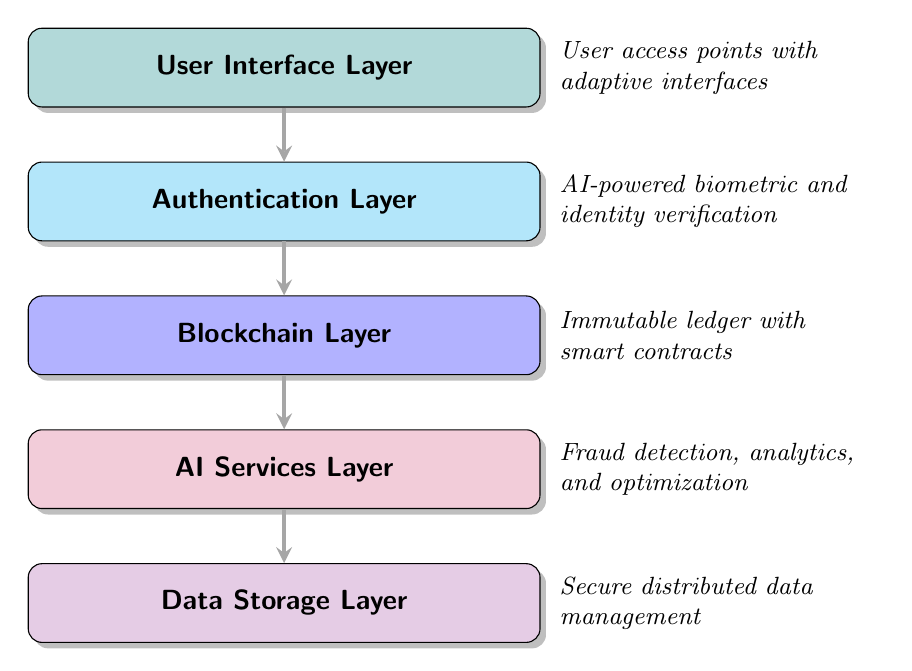
\begin{tikzpicture}[
  node distance=0.7cm,
  box/.style={
    draw, 
    fill=blue!10, 
    minimum width=6.5cm, 
    minimum height=1cm, 
    rounded corners=5pt, 
    drop shadow, 
    font=\sffamily\bfseries,
    align=center
  },
  arrow/.style={
    -stealth, 
    line width=1.5pt, 
    draw=gray!70
  }
]
% Layers - enhanced structure with better styling
\node[box, fill=teal!30] (l5) at (0,0) {User Interface Layer};
\node[box, fill=cyan!30] (l4) at (0,-1.7) {Authentication Layer};
\node[box, fill=blue!30] (l3) at (0,-3.4) {Blockchain Layer};
\node[box, fill=purple!20] (l2) at (0,-5.1) {AI Services Layer};
\node[box, fill=violet!20] (l1) at (0,-6.8) {Data Storage Layer};

% Connections with better arrows
\draw[arrow] (l5) -- (l4);
\draw[arrow] (l4) -- (l3);
\draw[arrow] (l3) -- (l2);
\draw[arrow] (l2) -- (l1);

% Add layer descriptions on the right
\node[text width=4cm, align=left, font=\small\itshape] at (5.5,0) {User access points with adaptive interfaces};
\node[text width=4cm, align=left, font=\small\itshape] at (5.5,-1.7) {AI-powered biometric and identity verification};
\node[text width=4cm, align=left, font=\small\itshape] at (5.5,-3.4) {Immutable ledger with smart contracts};
\node[text width=4cm, align=left, font=\small\itshape] at (5.5,-5.1) {Fraud detection, analytics, and optimization};
\node[text width=4cm, align=left, font=\small\itshape] at (5.5,-6.8) {Secure distributed data management};
\end{tikzpicture}
\caption{Layered Architecture for AI-Blockchain Voting System}
\label{fig:architecture}
\end{figure}

\subsubsection{User Interface Layer}
The User Interface Layer represents the various access points through which voters, administrators, and observers interact with the system. This layer could incorporate AI-driven adaptive interfaces that adjust to user capabilities and preferences, enhancing accessibility and user experience.

\subsubsection{Authentication Layer}
The Authentication Layer verifies voter identity and eligibility. AI capabilities in this layer include facial recognition, fingerprint matching, behavioral biometrics, and document analysis. These technologies could be integrated with blockchain-based zero-knowledge proofs to verify eligibility without exposing personal data.

\subsubsection{Blockchain Layer}
The Blockchain Layer provides the secure, transparent, and immutable record of the voting process. This layer includes smart contracts that encode voting rules, consensus mechanisms to validate transactions, and the distributed ledger that stores encrypted votes. AI can enhance this layer through intelligent contract verification, dynamic consensus optimization, and adaptive security measures.

\subsubsection{AI Services Layer}
The AI Services Layer provides intelligent functionality across the system. Key components include fraud detection algorithms, pattern analysis for system optimization, anomaly detection to identify potential security breaches, and predictive models for resource allocation and turnout estimation. This layer connects to the blockchain to access data while maintaining privacy and security.

\subsubsection{Data Storage Layer}
The Data Storage Layer manages system data with an emphasis on security and privacy. It includes distributed storage for public data, encrypted databases for sensitive information, backup systems, and comprehensive audit logs. AI can enhance this layer through intelligent data management, automated backup strategies, and optimized storage allocation.

\section{AI-Blockchain Integration Points}
Our framework identifies key integration points where AI and blockchain technologies synergistically enhance voting systems. Figures~\ref{fig:integration} and~\ref{fig:workflow} illustrate these integration points and their information flows.

\begin{figure}[!htb]
\centering
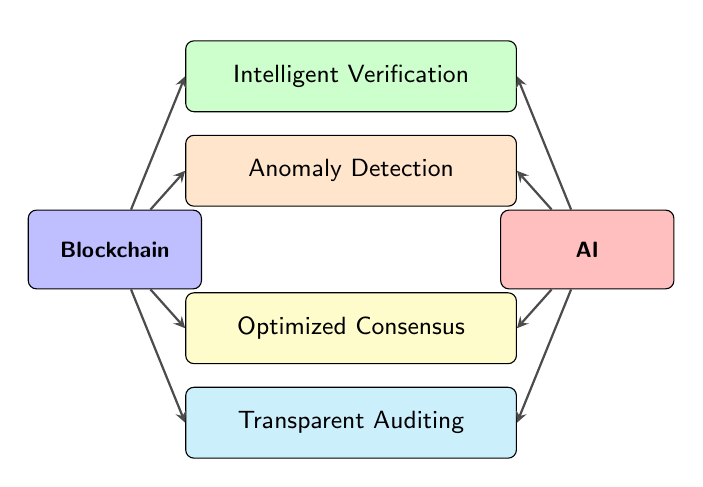
\begin{tikzpicture}[
  node distance=1.4cm,
  tech/.style={
    rectangle, 
    draw=black, 
    fill=#1!25, 
    minimum width=2.2cm, 
    minimum height=1cm, 
    rounded corners=3pt,
    font=\sffamily\bfseries\footnotesize,
    align=center
  },
  integration/.style={
    rectangle, 
    draw=black, 
    fill=#1!20, 
    minimum width=4.2cm, 
    minimum height=0.9cm, 
    rounded corners=3pt,
    font=\sffamily\small,
    align=center
  },
  connection/.style={
    -stealth, 
    thick, 
    draw=black!70
  }
]

% Left and right main technologies
\node[tech=blue] (bc) at (0,0) {Blockchain};
\node[tech=red] (ai) at (6,0) {AI};

% Middle stack
\node[integration=green] (iv) at (3,2.2) {Intelligent Verification};
\node[integration=orange] (ad) at (3,1) {Anomaly Detection};
\node[integration=yellow] (oc) at (3,-1) {Optimized Consensus};
\node[integration=cyan] (ta) at (3,-2.2) {Transparent Auditing};

% Arrows from tech to integration
\draw[connection] (bc) -- (iv.west);
\draw[connection] (ai) -- (iv.east);

\draw[connection] (bc) -- (ad.west);
\draw[connection] (ai) -- (ad.east);

\draw[connection] (bc) -- (oc.west);
\draw[connection] (ai) -- (oc.east);

\draw[connection] (bc) -- (ta.west);
\draw[connection] (ai) -- (ta.east);

% Feature label
\node[font=\scriptsize, anchor=west] at (0,2.7) {};

\end{tikzpicture}
\caption{Integration points between AI and blockchain technologies in voting systems}
\label{fig:integration}
\end{figure}






\subsubsection{Intelligent Verification}
At this integration point, AI-powered identity verification technologies (facial recognition, document verification) work with blockchain-based zero-knowledge proofs to create a secure, private authentication process. The AI verifies the voter's physical identity, while the blockchain confirms eligibility without revealing personal information.

\subsubsection{Anomaly Detection}
The Anomaly Detection integration point combines AI fraud detection algorithms with blockchain's immutable record to identify and prevent fraudulent activities. Machine learning models analyze patterns in voting data and blockchain transactions to flag unusual behaviors, while the blockchain provides a transparent, tamper-proof record of these alerts for investigation.

\subsubsection{Optimized Consensus}
This integration point uses AI predictive analytics to optimize blockchain consensus processes. By analyzing network conditions, voter patterns, and system performance, AI can adjust consensus parameters dynamically to maintain security and efficiency during varying load conditions. This addresses one of blockchain's key limitations for voting applications—scalability during peak voting periods.

\subsubsection{Transparent Auditing}
The Transparent Auditing integration point combines blockchain's transparent record with AI's analytical capabilities to create trustworthy audit processes. Machine learning algorithms can detect statistical anomalies in voting data, while the blockchain ensures these analyses and their results are recorded immutably and available for public verification.

\subsection{Information Flow and System Processes}
The conceptual framework includes processes that span multiple layers and components. Fig. 3 illustrates a high-level view of information flow through the integrated system, highlighting the role of both AI and blockchain components.

\begin{figure}[!htb]
\raggedright
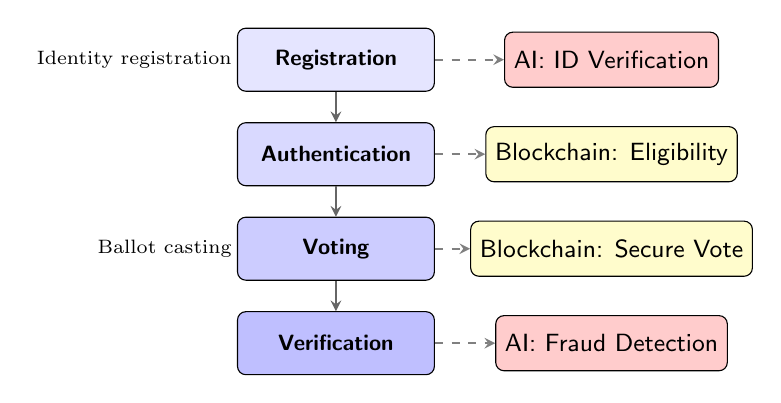
\begin{tikzpicture}[
  node distance=1.5cm,
  process/.style={
    rectangle, 
    draw=black, 
    fill=blue!#1, 
    minimum width=2.5cm, 
    minimum height=0.8cm, 
    rounded corners=3pt,
    font=\sffamily\bfseries\footnotesize,
    align=left
  },
  tech/.style={
    rectangle, 
    draw=black, 
    fill=#1!20, 
    minimum width=2.5cm, 
    minimum height=0.7cm, 
    rounded corners=3pt,
    font=\sffamily\small,
    align=left
  },
  flow/.style={
    -stealth, 
    line width=0.7pt, 
    draw=black!60
  },
  dashflow/.style={
    -stealth, 
    line width=0.7pt, 
    draw=black!50, 
    dashed
  }
]
% Process flow
\node[process=10] (reg) at (0,0) {Registration};
\node[process=15] (auth) at (0,-1.2) {Authentication};
\node[process=20] (vote) at (0,-2.4) {Voting};
\node[process=25] (verify) at (0,-3.6) {Verification};

% Technology
\node[tech=red] (ai1) at (3.5,0) {AI: ID Verification};
\node[tech=yellow] (bc1) at (3.5,-1.2) {Blockchain: Eligibility};
\node[tech=yellow] (bc2) at (3.5,-2.4) {Blockchain: Secure Vote};
\node[tech=red] (ai2) at (3.5,-3.6) {AI: Fraud Detection};

% Connections
\draw[flow] (reg) -- (auth);
\draw[flow] (auth) -- (vote);
\draw[flow] (vote) -- (verify);

\draw[dashflow] (reg) -- (ai1);
\draw[dashflow] (auth) -- (bc1);
\draw[dashflow] (vote) -- (bc2);
\draw[dashflow] (verify) -- (ai2);

% Descriptions
\node[font=\scriptsize, anchor=east] at (-1.2,0) {Identity registration};
\node[font=\scriptsize, anchor=east] at (-1.2,-2.4) {Ballot casting};
\end{tikzpicture}
\caption{Information flow in AI-blockchain voting system}
\label{fig:workflow}
\end{figure}

This information flow represents a conceptual process that integrates AI and blockchain components across various phases of the electoral process. It illustrates how these technologies could work together throughout the voting lifecycle, from registration to result verification.

\section{Potential Applications and Use Cases}
Based on our conceptual framework, we identify several promising applications and use cases for AI-blockchain integration in voting systems. These represent opportunities for researchers and practitioners to develop specific implementations that address key challenges in electronic voting.

\subsection{Intelligent Authentication and Verification}
Integrating AI-powered biometric authentication with blockchain-based eligibility verification represents a promising application area. This approach could provide strong security while maintaining voter privacy through:

\begin{itemize}
    \item \textbf{Multi-modal biometric verification:} Combining facial recognition, fingerprint scanning, and potentially voice recognition through AI algorithms to achieve higher accuracy than single-factor approaches. Joseph et al. \cite{b6} demonstrated that multi-modal approaches with liveness detection could significantly reduce false acceptance rates.
    
    \item \textbf{Document verification:} AI-powered computer vision and OCR technologies could authenticate identification documents in real-time, extracting and verifying information against registration databases while maintaining privacy.
    
    \item \textbf{Behavioral biometrics:} Advanced AI could analyze typing patterns, gesture dynamics, or other behavioral markers as an additional verification layer, particularly valuable for remote voting scenarios.
    
    \item \textbf{Zero-knowledge eligibility proofs:} These cryptographic techniques, recorded on the blockchain, could verify a voter's eligibility without revealing their identity, creating a privacy-preserving yet verifiable authentication process.
\end{itemize}

This application area addresses one of the fundamental challenges in electronic voting: how to verify voter identity securely while protecting privacy and preventing impersonation. As Balti et al. \cite{b2} emphasized, the robustness of authentication mechanisms is critical for maintaining the integrity of the voting process.

\subsection{Fraud Detection and Prevention}
AI and blockchain offer complementary strengths for detecting and preventing electoral fraud:

\begin{itemize}
    \item \textbf{Real-time anomaly detection:} AI algorithms could analyze voting patterns and system interactions to identify statistical outliers that might indicate fraud attempts. These could include unusual geographic distributions, timing patterns, or system access behaviors.
    
    \item \textbf{Duplicate vote prevention:} Blockchain's consensus mechanisms ensure each eligible voter can cast only one valid vote, while AI could help identify sophisticated attempts to circumvent these controls, as demonstrated by Sliusar et al. \cite{b4}.
    
    \item \textbf{Smart contract monitoring:} AI systems could continuously monitor smart contract execution to detect potential exploits or unexpected behaviors that might indicate an attack on the voting system.
    
    \item \textbf{Network security:} AI-powered intrusion detection systems could protect blockchain nodes from denial-of-service attacks or unauthorized access attempts during critical voting periods.
\end{itemize}

As Singh et al. \cite{b5} demonstrated, machine learning-based intrusion detection can significantly enhance the security of blockchain voting systems, particularly when the models are trained on election-specific attack patterns. Additionally, Tandon et al. \cite{b3} highlighted how decentralized blockchain architectures with proper consensus mechanisms can inherently resist many forms of electoral manipulation.

\subsection{Adaptive User Interfaces and Accessibility}
AI could enhance the inclusivity and usability of blockchain voting systems through:

\begin{itemize}
    \item \textbf{Adaptive interfaces:} Machine learning algorithms could adjust the user interface based on user capabilities, preferences, and device characteristics, making the system more accessible to voters with different needs, as noted by Edoo et al. \cite{b7} in their mobile voting platform.
    
    \item \textbf{Natural language processing:} AI could enable voice-controlled interfaces and multilingual support, reducing barriers for voters with limited literacy or physical disabilities.
    
    \item \textbf{Personalized assistance:} AI chatbots or virtual assistants could guide voters through the registration and voting process, providing context-specific help without compromising ballot secrecy.
    
    \item \textbf{Accessibility verification:} AI systems could automatically test voting interfaces against accessibility standards, identifying and suggesting improvements to ensure compliance.
\end{itemize}

These applications address a critical gap in many existing blockchain voting systems: accessibility and usability for diverse voter populations. By leveraging AI to enhance the user experience, these systems could become more inclusive while maintaining the security benefits of blockchain. Indukuri et al. \cite{b8} emphasized the importance of usability in democratic environments, noting that even technically sound voting systems may fail if voters find them difficult to use.

\subsection{Transparent Auditing and Result Verification}
The combination of AI analytics with blockchain's immutable record could create powerful tools for election integrity:

\begin{itemize}
    \item \textbf{Statistical verification:} Machine learning models could analyze voting results to identify statistically improbable patterns that might indicate manipulation or system errors, while the blockchain provides a transparent record of these analyses.
    
    \item \textbf{Automated auditing:} AI could automate parts of the post-election audit process, analyzing the blockchain record to verify that all votes were properly recorded and counted without revealing individual vote choices.
    
    \item \textbf{Explainable verification:} AI systems could generate human-understandable explanations of verification processes, helping voters, officials, and observers understand how the integrity of the election was maintained.
    
    \item \textbf{Continuous monitoring:} Rather than just post-election audits, AI could enable continuous monitoring of the voting system, identifying and addressing potential issues in real-time while recording these actions on the blockchain for transparency.
\end{itemize}

These applications address the critical need for public trust in electronic voting systems by combining the analytical power of AI with the transparency and immutability of blockchain. Khudoykulov et al. \cite{b1} identified transparency and trust as key challenges in blockchain voting systems, suggesting that enhanced verification mechanisms could help address these concerns.

\section{Challenges and Limitations}
Despite the promising opportunities for AI-blockchain integration in voting systems, significant challenges and limitations must be addressed before widespread implementation becomes feasible.

\subsection{Technical Challenges}
Several technical hurdles currently limit the practical implementation of integrated AI-blockchain voting systems:

\begin{itemize}
    \item \textbf{Scalability limitations:} Blockchain networks face significant throughput constraints compared to traditional databases. Current public blockchains like Ethereum can process only 15-30 transactions per second, insufficient for large-scale elections with millions of voters voting within a short timeframe, as noted by Singh et al. \cite{b5}.
    
    \item \textbf{Energy consumption:} Many blockchain consensus mechanisms, particularly Proof-of-Work, consume substantial energy. While more efficient alternatives exist, balancing energy efficiency with security remains challenging for voting applications, as identified by Sliusar et al. \cite{b4}.
    
    \item \textbf{Integration complexity:} Effectively integrating AI and blockchain systems requires addressing fundamental differences in processing models, data storage, and system architecture. This integration adds significant complexity to system design and implementation, as demonstrated by Edoo et al. \cite{b7} in their microservices approach.
    
    \item \textbf{AI model security:} AI models themselves can be vulnerable to adversarial attacks, where specially crafted inputs cause the model to make incorrect predictions. For voting applications, such vulnerabilities could compromise critical functions like voter authentication or fraud detection, according to Joseph et al. \cite{b6}.
    
    \item \textbf{Consensus mechanism selection:} Choosing appropriate consensus mechanisms for voting systems involves complex trade-offs between security, performance, and energy efficiency. Tandon et al. \cite{b3} highlighted the strengths and weaknesses of Proof of Work in their E-Matdaan system, noting that alternative approaches might be more suitable for certain voting scenarios.
\end{itemize}

\subsection{Data Privacy and Security Concerns}
Voting systems must maintain the highest standards of privacy and security, presenting specific challenges for AI-blockchain integration:

\begin{itemize}
    \item \textbf{Biometric data protection:} AI-powered authentication often relies on sensitive biometric data. Storing and processing this data securely while maintaining its usefulness for verification presents significant privacy challenges, as recognized by Joseph et al. \cite{b6} in their facial recognition system.
    
    \item \textbf{Blockchain privacy limitations:} While blockchains provide transparency, excessive transparency can compromise voter privacy. Techniques like zero-knowledge proofs and homomorphic encryption add complexity and processing overhead, as explored by Singh et al. \cite{b5}.
    
    \item \textbf{Re-identification risks:} Even with privacy-preserving techniques, the combination of multiple data points recorded on the blockchain might allow for voter re-identification through sophisticated analysis, a concern highlighted by Khudoykulov et al. \cite{b1} in their analysis of open issues in blockchain-based voting.
    
    \item \textbf{Data management across borders:} International or diaspora voting introduces questions about data sovereignty and cross-border data transfers, particularly for sensitive biometric information used in AI authentication, a concern highlighted by Edoo et al. \cite{b7} in their mobile voting solution.
\end{itemize}

\subsection{Regulatory and Legal Challenges}
The implementation of AI-blockchain voting systems faces significant regulatory and legal hurdles:

\begin{itemize}
    \item \textbf{Regulatory uncertainty:} Many jurisdictions lack comprehensive regulatory frameworks for either blockchain-based voting or AI in electoral systems, creating legal uncertainty for implementation, as noted by Sliusar et al. \cite{b4}.
    
    \item \textbf{Compliance with electoral laws:} Existing electoral laws were generally written with paper-based voting in mind and may not easily accommodate blockchain or AI technologies without legislative updates.
    
    \item \textbf{Certification standards:} The lack of established certification standards specifically for AI-blockchain voting systems makes it difficult to validate their security, reliability, and compliance with electoral requirements.
    
    \item \textbf{Liability and accountability:} Determining responsibility when issues arise in AI-driven decisions or blockchain-based recording presents complex legal questions that current frameworks may not adequately address.
\end{itemize}

\subsection{Ethical and Social Considerations}
Beyond technical and legal challenges, the integration of AI with blockchain for voting raises important ethical and social questions:

\begin{itemize}
    \item \textbf{Digital divide:} Technological solutions may disadvantage voters without access to or familiarity with required devices and interfaces, potentially disenfranchising portions of the electorate, a concern raised by Singh et al. \cite{b5}.
    
    \item \textbf{Algorithmic bias:} AI systems may exhibit bias in authentication or fraud detection across demographic groups if not properly designed and tested with diverse data, as Joseph et al. \cite{b6} emphasized in their authentication system.
    
    \item \textbf{Transparency vs. comprehensibility:} While blockchain provides technical transparency, both blockchain and AI technologies may appear as "black boxes" to most voters, potentially undermining trust rather than enhancing it, according to Edoo et al. \cite{b7}.
    
    \item \textbf{Democratic oversight:} Determining who controls, audits, and certifies these systems raises fundamental questions about democratic oversight and the role of technology in electoral processes, an issue identified by Indukuri et al. \cite{b8} in their analysis of blockchain voting in democratic environments.
    
    \item \textbf{Coercion in remote voting:} Remote voting, even with blockchain and AI security measures, remains vulnerable to coercion in unsupervised environments, a concern highlighted by Balti et al. \cite{b2} in their analysis of security considerations for blockchain-based voting.
\end{itemize}

These challenges highlight the need for careful, interdisciplinary approaches to AI-blockchain integration in voting that consider not only technical feasibility but also legal compliance, ethical implications, and social impact.

\section{Research Gaps and Future Directions}
Based on our analysis of the current state of AI-blockchain integration in voting systems and the identified challenges, we propose several key areas for future research and development.

\subsection{Technical Research Opportunities}
Several technical areas require further research to advance AI-blockchain integration in voting systems:

\begin{itemize}
    \item \textbf{Scalable blockchain architectures:} Developing high-throughput blockchain architectures specifically designed for voting applications, potentially through layer-2 scaling solutions, sharding, or optimized consensus mechanisms tailored to electoral requirements.
    
    \item \textbf{Quantum-resistant cryptography:} Research into quantum-resistant algorithms for blockchain voting to ensure long-term security as quantum computing advances. This includes both transaction security and the protection of historical voting records.
    
    \item \textbf{Privacy-preserving AI:} Advancing techniques for AI to process biometric and behavioral data without compromising privacy, including federated learning, differential privacy, and secure multi-party computation for authentication and fraud detection.
    
    \item \textbf{Adversarial resilience:} Developing AI models resistant to adversarial attacks, ensuring that authentication and fraud detection systems cannot be manipulated through specially crafted inputs designed to cause incorrect classifications.
    
    \item \textbf{On-chain AI verification:} Creating mechanisms for blockchain-based verification of AI model integrity and decision processes, ensuring that the AI components cannot be tampered with and their operations remain transparent.
\end{itemize}

\subsection{System Integration and Standards}
Standardization and integration frameworks represent crucial areas for advancing the field:

\begin{itemize}
    \item \textbf{Reference architectures:} Developing open reference architectures for integrating AI with blockchain in voting applications, providing guidelines for component interaction, data flow, and security requirements.
    
    \item \textbf{Interoperability standards:} Creating standards for data exchange between AI and blockchain components, enabling different implementations to work together cohesively and facilitating modular system design.
    
    \item \textbf{Testing and certification frameworks:} Establishing comprehensive testing methodologies and certification criteria specifically for AI-blockchain voting systems, addressing their unique characteristics and risk profiles.
    
    \item \textbf{Benchmarking datasets:} Creating standardized, diverse datasets for training and testing AI components of voting systems, particularly for authentication and fraud detection, while addressing privacy concerns in dataset creation.
\end{itemize}

\subsection{Implementation and Governance Studies}
Research on practical implementation and governance models is essential for real-world applications:

\begin{itemize}
    \item \textbf{Decentralized governance models:} Developing and evaluating governance frameworks for AI-blockchain voting systems that balance technical expertise, democratic oversight, and public accountability in system management.
    
    \item \textbf{Progressive implementation strategies:} Researching approaches for gradual adoption, such as using AI-blockchain systems alongside traditional methods before full transition, with appropriate evaluation metrics for comparative assessment.
    
    \item \textbf{Cross-border implementation:} Studying the legal, technical, and operational challenges of implementing these systems across jurisdictional boundaries for international or diaspora voting.
    
    \item \textbf{Risk assessment frameworks:} Creating comprehensive methodologies for assessing the security, privacy, and social risks of AI-blockchain voting implementations in different contexts.
\end{itemize}

\subsection{Human Factors and Accessibility Research}
Understanding human interaction with these systems represents a critical and often overlooked research area:

\begin{itemize}
    \item \textbf{Universal design approaches:} Researching design methodologies that ensure AI-blockchain voting systems are accessible to all voters, including those with disabilities, limited technological literacy, or language barriers.
    
    \item \textbf{Trust formation studies:} Investigating how voters form trust judgments about AI-blockchain voting systems and identifying design features that enhance legitimate trust while discouraging misplaced trust.
    
    \item \textbf{Usability across demographics:} Studying how different demographic groups interact with these systems and developing adaptive interfaces that accommodate diverse needs without compromising security or privacy.
    
    \item \textbf{Voter education strategies:} Researching effective approaches for educating voters about AI-blockchain voting systems, balancing technical accuracy with comprehensibility.
\end{itemize}

\subsection{Ethical and Societal Impact Research}
Research on ethical implications and societal impacts will be crucial for responsible development:

\begin{itemize}
    \item \textbf{Algorithmic fairness in voting:} Developing methodologies for identifying and mitigating bias in AI components of voting systems, with particular attention to authentication and fraud detection algorithms.
    
    \item \textbf{Digital divide mitigation:} Researching strategies to ensure AI-blockchain voting systems do not disenfranchise voters with limited technological access or literacy.
    
    \item \textbf{Transparency mechanisms:} Developing approaches for making complex AI-blockchain operations understandable to non-technical stakeholders, including voters, officials, and observers.
    
    \item \textbf{Long-term societal impact:} Studying the potential effects of AI-blockchain voting on democratic participation, public trust in institutions, and civic engagement.
\end{itemize}

These research directions address critical gaps in the current understanding of AI-blockchain integration for voting systems and provide a roadmap for advancing the field toward more secure, accessible, and trustworthy implementations.

\section{Conclusion}
This study has examined the potential integration of artificial intelligence with blockchain technology to enhance electronic voting systems. Through a comprehensive literature review, we have identified the current state of both technologies in electoral applications, analyzed their complementary strengths, and proposed a conceptual framework for their integration.

The integration of AI with blockchain offers promising opportunities to address key challenges in electronic voting, including secure authentication, fraud detection, system optimization, and transparent auditing. AI can enhance blockchain's capabilities through intelligent verification, anomaly detection, consensus optimization, and automated auditing, while blockchain provides the secure, transparent foundation necessary for trustworthy voting systems.

However, significant challenges remain before widespread implementation becomes feasible. Technical limitations such as scalability, energy efficiency, and integration complexity must be addressed. Data privacy concerns, particularly regarding biometric information used in AI authentication, require careful consideration. Regulatory frameworks need updating to accommodate these technologies, and ethical questions about accessibility, algorithmic bias, and democratic oversight demand thoughtful responses.

Our analysis has identified several research gaps and future directions, including technical advances in scalable blockchain architectures and privacy-preserving AI, standardization efforts for interoperability and certification, governance studies for implementation strategies, human factors research on accessibility and trust, and ethical investigations of algorithmic fairness and digital divide concerns.

As societies increasingly explore digital solutions for democratic processes, the thoughtful integration of AI with blockchain has the potential to create voting systems that are more secure, accessible, and trustworthy than either traditional paper-based methods or first-generation electronic systems. However, realizing this potential requires interdisciplinary collaboration among technologists, election officials, legal experts, ethicists, and citizens to ensure that these systems serve democratic values rather than undermining them.

By providing a conceptual framework and research roadmap, this study aims to contribute to the development of voting technologies that leverage the complementary strengths of AI and blockchain while addressing their limitations, ultimately supporting the evolution of more robust democratic systems in the digital age.

\section{Novel Approaches and Future Implementations}
Building upon the research gaps and opportunities identified in this paper, we propose several novel approaches that have not been implemented in current AI-blockchain voting systems but represent promising avenues for future development. These concepts extend beyond existing research to address fundamental challenges in electronic voting while leveraging emerging technologies.

\subsection{Federated Biometric Verification with Threshold Cryptography}
Current biometric verification approaches in voting systems typically store templates in centralized databases or on blockchain, creating potential privacy vulnerabilities. We propose a novel approach combining federated learning with threshold cryptography for fully distributed biometric verification.

In this approach, biometric templates would be cryptographically sharded across multiple nodes using threshold schemes, where no single node holds a complete template. An AI-driven federated learning system would train verification models across these distributed fragments without reconstructing complete templates, maintaining privacy while enabling accurate verification.

The verification process would occur across the distributed network, with each node contributing partial verification without accessing complete biometric data. This approach would require:

\begin{itemize}
    \item A novel application of threshold cryptography specifically designed for biometric data fragmentation
    \item Custom federated learning protocols optimized for partial biometric matching
    \item Blockchain-based coordination of the distributed verification process
    \item Specialized zero-knowledge proofs to verify the integrity of the federated system
\end{itemize}

This approach would significantly enhance privacy compared to existing biometric systems by mathematically ensuring that no complete biometric template exists in any single location while still enabling high-accuracy verification.

\subsection{Neurosymbolic AI for Transparent Election Auditing}
Traditional AI approaches to election auditing rely heavily on "black box" neural networks that provide limited explainability, undermining trust in the audit process. We propose a novel neurosymbolic AI approach—combining neural networks with symbolic reasoning—to create inherently transparent and explainable audit mechanisms.

This system would:

\begin{itemize}
    \item Extract statistical patterns from voting data using neural components
    \item Transform these patterns into formal logical expressions through symbolic reasoning
    \item Apply formal verification methods to these expressions to detect potential anomalies
    \item Generate human-readable explanations of its findings with logical justification
    \item Record both findings and reasoning processes immutably on the blockchain
\end{itemize}

Unlike traditional "black box" AI, this neurosymbolic approach would produce audit results with clear, verifiable reasoning chains that election officials, observers, and voters could follow and validate. This addresses the critical transparency gap in current AI-based audit systems while maintaining the pattern recognition capabilities needed for effective fraud detection.

The system would be designed to reason about election data at multiple levels of abstraction, from individual transaction patterns to statistical distributions of voting behavior, providing a comprehensive audit capability that doesn't compromise on explainability.

\subsection{Adaptive Privacy-Utility Optimization through Contextual Bandits}
Electronic voting systems face an inherent tension between transparency (necessary for verification) and privacy (necessary for ballot secrecy). Current approaches use static privacy mechanisms that don't adapt to changing conditions during an election.

We propose a novel approach using contextual bandit algorithms—a form of reinforcement learning—to dynamically optimize the privacy-utility tradeoff throughout the election process. This system would:

\begin{itemize}
    \item Continuously monitor the information environment surrounding the election
    \item Assess potential privacy risks from data already published on the blockchain
    \item Dynamically adjust differential privacy parameters for subsequent data releases
    \item Maximize transparency where safe while increasing privacy protections where needed
    \item Learn optimal privacy-utility policies through simulation before deployment
\end{itemize}

This approach represents a significant advancement over current static privacy mechanisms, as it would adapt to emerging conditions—such as attempted de-anonymization attacks or unexpected correlations in published data—to maintain optimal privacy protection throughout the election process.

The system would leverage blockchain's immutable record to document all privacy parameter adjustments, ensuring that the adaptation process itself remains transparent and verifiable while the private ballot data stays protected.

\subsection{Cognitive Digital Twins for System Resilience}
Current voting systems typically employ static security models that cannot adapt to emerging threats during an election. We propose developing "cognitive digital twins"—AI-driven simulations of the entire voting system that run parallel to the actual system—to anticipate vulnerabilities and proactively adjust defenses.

These digital twins would:

\begin{itemize}
    \item Continuously model the voting system's state, including blockchain transactions, network traffic, and user interactions
    \item Simulate potential attack vectors in a sandboxed environment
    \item Deploy counter-measures to the live system before attacks materialize
    \item Document all security adjustments on the blockchain for transparent security governance
    \item Learn from actual and simulated attacks to improve future resilience
\end{itemize}

This approach would move beyond reactive security to create anticipatory system defense, significantly enhancing resilience against zero-day attacks and sophisticated threats. By maintaining digital twins of critical system components, the voting system could simulate the impact of potential attacks without risking actual election integrity.

The approach represents a novel application of digital twin technology, typically used in engineering contexts, to the cybersecurity domain of voting systems. Combined with blockchain's immutable record, it would create unprecedented transparency in security operations while maintaining robust protection against emerging threats.

\begin{thebibliography}{8}
\bibitem{b1}
Z. Khudoykulov, U. Tojiakbarova, S. Bozorov and D. Ourbonalieva, ``Blockchain Based E-Voting System: Open Issues and Challenges,'' in {\it International Conference on Information Science and Communications Technologies (ICISCT)}, Tashkent, Uzbekistan, 2021, pp. 1-5, doi: 10.1109/ICISCT52966.2021.9670245.

\bibitem{b2}
A. Balti, A. Prabhu, S. Shahi, S. Dahifale and V. Maheta, ``A Decentralized and Immutable E-Voting System using Blockchain,'' in {\it International Conference on Sustainable Computing and Smart Systems (ICSCSS)}, Coimbatore, India, 2023, pp. 1434-1439, doi: 10.1109/ICSCSS57650.2023.10169552.

\bibitem{b3}
S. Tandon, N. Singh, S. Porwal, Satiram and A. K. Maurya, ``E-Matdaan: A Blockchain based Decentralized E-Voting System,'' in {\it IEEE Students Conference on Engineering and Systems (SCES)}, Prayagraj, India, 2022, pp. 1-6, doi: 10.1109/SCES55490.2022.9887759.

\bibitem{b4}
V. Sliusar, P. Fyodorov, A. Fyodorov, V. Pascari, and A. Volkov, ``Blockchain Technology Application for Electronic Voting Systems,'' in {\it IEEE Conference of Russian Young Researchers in Electrical and Electronic Engineering (ElConRus)}, 2021, pp. 2257-2261, doi: 10.1109/ElConRus51938.2021.9396400.

\bibitem{b5}
S. Singh, A. Singh, S. Verma, and R. K. Dwivedi, ``Designing a Blockchain-Enabled Methodology for Secure Online Voting System,'' in {\it International Conference on Intelligent Data Communication Technologies and Internet of Things (IDCIoT)}, 2023, pp. 178-184, doi: 10.1109/IDCIoT56793.2023.10053410.

\bibitem{b6}
S. Joseph, P. Pandey, M. Khari, K. Kumar, and P. P. Singh, ``Ether Vote: Revolutionizing Elections with Blockchain-Powered Electronic Voting System,'' in {\it 3rd International Conference on Smart Generation Computing, Communication and Networking (SMART GENCON)}, 2023, pp. 1-7, doi: 10.1109/SMARTGENCON60755.2023.10442887.

\bibitem{b7}
J. B. A. Edoo, R. K. Sungkur, J. M. Gómez, H. Precht, and S. Rudolph, ``Mauvote: A Novel Mobile Electronic Voting System Using Blockchain,'' in {\it International Conference on Next Generation Computing Applications (NextComp)}, 2024, pp. 1-6, doi: 10.1109/NextComp63004.2024.10779646.

\bibitem{b8}
N. S. Varma Indukuri, S. Reddy Eguram, A. Nichena, S. Ulvalapudi and R. Gajula, ``Blockchain-based Voting System in a Democratic Environment,'' in {\it Second International Conference on Augmented Intelligence and Sustainable Systems (ICAISS)}, Trichy, India, 2023, pp. 1312-1316, doi: 10.1109/ICAISS58487.2023.10250609.
\end{thebibliography}

\end{document}


